% ****** Start of file apssamp.tex ******
%
%   This file is part of the APS files in the REVTeX 4.2 distribution.
%   Version 4.2a of REVTeX, December 2014
%
%   Copyright (c) 2014 The American Physical Society.
%
%   See the REVTeX 4 README file for restrictions and more information.
%
% TeX'ing this file requires that you have AMS-LaTeX 2.0 installed
% as well as the rest of the prerequisites for REVTeX 4.2
%
% See the REVTeX 4 README file
% It also requires running BibTeX. The commands are as follows:
%
%  1)  latex apssamp.tex
%  2)  bibtex apssamp
%  3)  latex apssamp.tex
%  4)  latex apssamp.tex
%
\documentclass[%
 reprint,
%superscriptaddress,
%groupedaddress,
%unsortedaddress,
%runinaddress,
%frontmatterverbose, 
%preprint,
%preprintnumbers,
%nofootinbib,
%nobibnotes,
%bibnotes,
 amsmath,amssymb,
 aps,
prc,
%prb,
%rmp,
%prstab,
%prstper,
%floatfix,
]{revtex4-2}

\usepackage{graphicx}% Include figure files
\usepackage{dcolumn}% Align table columns on decimal point
\usepackage{bm}% bold math
\usepackage{hyperref}% add hypertext capabilities
\usepackage{tikz}
\usetikzlibrary{positioning,arrows.meta}
\usepackage{helvet}
\usepackage{sansmath}
%\usepackage[mathlines]{lineno}% Enable numbering of text and display math
%\linenumbers\relax % Commence numbering lines

%\usepackage[showframe,%Uncomment any one of the following lines to test 
%%scale=0.7, marginratio={1:1, 2:3}, ignoreall,% default settings
%%text={7in,10in},centering,
%%margin=1.5in,
%%total={6.5in,8.75in}, top=1.2in, left=0.9in, includefoot,
%%height=10in,a5paper,hmargin={3cm,0.8in},
%]{geometry}

\begin{document}


\title{\texorpdfstring{Constraining the Low-$\bm{p_T}$ $\bm{\eta/\pi^0}$ Ratio for Direct-Photon Analyses with Blast-Wave Fits to $\bm{\pi}$, $\bm{K}$, and $\bm{p}$ Spectra}{Constraining the Low-p\_T eta/pi0 Ratio for Direct-Photon Analyses with Blast-Wave Fits to pi, K, and p Spectra}}% Force line breaks with \\
%\thanks{A footnote to the article title}%

\author{Klaus Reygers}%
 \email{reygers@physi.uni-heidelberg.de}
\affiliation{Physikalisches Institut, Universit\"{a}t Heidelberg, 69120 Heidelberg, Germany}
\author{Andreas Kirchner}
\email{andreas.kirchner@duke.edu}
\affiliation{Department of Physics, Duke University, Durham, North Carolina 27708, USA}
\affiliation{Institut f\"{u}r Theoretische Physik, Universit\"{a}t Heidelberg, 69120 Heidelberg, Germany}
\author{Aleksas Mazeliauskas}%
 \email{a.mazeliauskas@thpys.uni-heidelberg.de}
\affiliation{Institut f\"{u}r Theoretische Physik, Universit\"{a}t Heidelberg, 69120 Heidelberg, Germany}

%\collaboration{MUSO Collaboration}%\noaffiliation

%\collaboration{CLEO Collaboration}%\noaffiliation

\date{\today}% It is always \today, today,
             %  but any date may be explicitly specified

\begin{abstract}
We predict the $\eta/\pi^0$ ratio at low $p_T$ ($p_T \lesssim 3~\mathrm{GeV}/c$) using the measured charged $K/\pi$ ratio and model input from a blast-wave framework with feeddown contributions. This approach can provide improved, data-constrained background estimates for direct-photon and dilepton measurements in heavy-ion collisions. In this approach, the explicit modeling of radial flow and hadronic feeddown enables an uncertainty estimate for the low-$p_T$ extrapolation of the $\eta/\pi^0$ ratio. Using central Pb--Pb collisions at $\sqrt{s_{NN}}=2.76$~TeV as an example, we find that the $\eta$-related decay-photon uncertainty at $p_T \approx 1~\mathrm{GeV}/c$ is of order 10\% of the expected direct-photon signal.
\end{abstract}

%\keywords{Suggested keywords}%Use showkeys class option if keyword
                              %display desired
\maketitle

\section{Introduction}
Ultrarelativistic collisions of nuclei are a unique laboratory for studying quantum chromodynamics (QCD) at extreme temperatures and densities. These collisions are widely interpreted as creating a quark-gluon plasma (QGP), i.e., an approximately thermalized medium whose relevant degrees of freedom are quarks and gluons \cite{Busza:2018rrf}. The QGP expands, cools, and hadronizes at a temperature of about 156~MeV~\cite{Borsanyi:2018grb,HotQCD:2018pds}, which coincides with the experimentally extracted chemical freeze-out temperature~\cite{Andronic:2017pug}. Real and virtual photons (dileptons) are a key probe of the medium as they are produced in all stages of the collision and are not affected by hadronization. Thermal photons and dileptons are of particular interest since their spectrum reflects the temperature of the medium. 

Experimentally, one measures direct photons by statistically subtracting the large background of photons from hadron decays. The largest contribution to the decay-photon background comes from the $\pi^0 \to \gamma \gamma$ decay (about 83--88\%), followed by the $\eta \to \gamma \gamma$ decay (about 10--15\%). Together, the $\pi^0$ and the $\eta$ contribute about 98\% to the decay-photon background. The third-largest contribution, up to about 1--2\%, comes from the decays $\omega \to \pi^0 \gamma (\eta \gamma)$. All other hadron decays are practically negligible~\cite{ALICE:2015xmh}. In the case of dileptons, a similar experimental approach of subtracting a ``cocktail'' of known background sources from the total number of correlated $e^+e^-$ pairs is taken. Here the Dalitz decays $\pi^0 \to \gamma e^+e^-$ and $\eta \to \gamma e^+e^-$ are the most important background sources at low $e^+e^-$ invariant masses.

For real photons, the low transverse momentum region ($p_T \lesssim 3\,\mathrm{GeV}/c$) is of special interest due to the significant contribution of thermal photons from the QGP phase and the subsequent hadron gas phase~\cite{David:2019wpt}. The yield of background photons from the two-photon decay of the $\eta$ meson is expected to be similar in magnitude or larger than the signal of thermal photons. However, at low $p_T$ the measurement of the $\eta$ meson is difficult and typically associated with large uncertainties. Therefore, various approaches to model the $p_T$ spectrum of the $\eta$ meson were employed in the past. No approach yet combines experimental constraints with decay feeddown in a unified framework.

In this paper, we present an approach to model the $\eta/\pi^0$ ratio at low $p_T$ using measured charged $K/\pi$ input and blast-wave modeling of hadron spectra, including decay contributions from short-lived hadrons \cite{Mazeliauskas:2019ifr}. Our central claim is that the new method enables improved control and reduction of the decay-cocktail uncertainties associated with the $\eta$ meson. This is expected to enable a more precise extraction of the direct-photon and low-mass dilepton signals in heavy-ion collisions.

\section{\boldmath Previous Approaches to Constraining Low-$p_T$ $\eta/\pi^0$}

Different approaches to model the $\eta/\pi^0$ ratio at low $p_T$ were used in previous measurements of direct photons in nucleus--nucleus collisions. In Pb--Pb collisions at $\sqrt{s_\mathrm{NN}} = 17.3\,\mathrm{GeV}$ at the CERN SPS, the WA98 experiment assumed $m_T$ scaling to estimate the $\eta/\pi^0$ ratio in the unmeasured low-$p_T$ region \cite{WA98:2000vxl}. The $m_T$ scaling hypothesis states that invariant hadron yields for different particle species have the same spectral shape as a function of $m_T = \sqrt{m^2+p_T^2}$ and only differ by an overall normalization factor \cite{Albrecht:1991zza}. The $m_T$ scaling hypothesis was also used in direct-photon measurements by the PHENIX experiment at RHIC \cite{PHENIX:2008uif}. At high collision energies, however, the strong collective radial flow of the medium is expected to give rise to significant deviations from $m_T$ scaling. At the LHC, the ALICE experiment considered the $m_T$ scaling prediction as a limiting case to estimate the systematic uncertainty of the $\eta/\pi^0$ ratio \cite{ALICE:2015xmh}. 

To take the effect of radial flow into account, the STAR experiment used a Tsallis blast-wave model to predict the $\eta/\pi^0$ ratio \cite{STAR:2016use}. More recently, Ren and Drees proposed a method to estimate the $\eta/\pi^0$ ratio in nucleus--nucleus (AA) collisions based on the assumption that $\eta/\pi^0$ as a function of $p_T$ is approximately independent of the collision energy over a wide range of energies \cite{Ren:2021pzi}. The effect of radial flow on the $\eta/\pi^0$ ratio is then modeled by multiplying the universal $\eta/\pi^0$ in proton--proton collisions by the ratio of the charged $K/\pi$ ratios in AA and pp collisions:
\begin{equation}
\left(\eta/\pi^0\right)_{\mathrm{AA}} =
\frac{\left(K/\pi\right)_{\mathrm{AA}}}{\left(K/\pi\right)_{\mathrm{pp}}}
\left(\eta/\pi^0\right)_{\mathrm{pp}}.
\end{equation}
This approach was used in a recent direct-photon measurement by the PHENIX experiment \cite{PHENIX:2022rsx}. 

Both the Tsallis blast-wave approach by the STAR experiment and the Ren--Drees method underline the importance of modeling the effect of radial flow for the prediction of the $\eta/\pi^0$ ratio. A blast-wave model approach, as used by STAR, can be improved by including the effect of decays of short-lived hadrons. This applies also to the method by Ren and Drees where kaons are used as a flow proxy for $\eta$. This implicitly assumes that the effect of resonance decays is similar for the $\eta/\pi^0$ ratio and the $K/\pi$ ratio. Moreover, the effect of radial flow depends on the mass of the particle. The mass difference between the kaon ($m_K = 494\,\mathrm{MeV}$) and the $\eta$ meson ($m_\eta = 548\,\mathrm{MeV}$) could therefore affect the accuracy of this method. We will compare the results of the Ren--Drees approach and our approach in this paper.

\section{\boldmath Method: Data-Driven $\eta/\pi^{0}$ from Measured $K/\pi$}

We determine the low-$p_T$ ($p_T \lesssim 3\,\mathrm{GeV}/c$) $\eta/\pi^0$ ratio in nucleus--nucleus collisions using the measured $K/\pi$ ratio in the same centrality class. This strategy exploits the fact that, unlike $\eta/\pi^0$, $K/\pi$ can be measured directly with high precision at low $p_T$. Our core method models hadron spectra within a blast-wave framework that includes resonance feeddown. In addition, we consider flow scaling as an alternative way to predict hadron spectra, which can be viewed as a generalization of $m_T$ scaling in the presence of strong radial flow. To our knowledge, this is the first application of this flow-scaling construction to model hadron spectra in heavy-ion collisions.

\subsection{Core Double-Ratio Method}
The central idea of our core double-ratio method is to determine the $\eta/\pi^0$ ratio by multiplying the model ratio $[(\eta/\pi^0)/(K/\pi)]_\mathrm{model}$ by the measured charged $K/\pi$ ratio. By constructing $\eta/\pi^0$ based on $K/\pi$, common normalization uncertainties cancel. The model parameters are determined by a fit to the measured $\pi$, $K$, and $p$ spectra. To keep this task manageable, we employ a blast-wave model \cite{Schnedermann:1992ra,Schnedermann:1993ws} based on the Cooper-Frye freeze-out prescription \cite{Cooper:1974mv}:
\begin{equation}
\left(\eta/\pi^0\right)_{\mathrm{AA}}
=
\frac{\left(\eta/\pi^0\right)_{\mathrm{blast\text{-}wave}}}
     {\left(K/\pi\right)_{\mathrm{blast\text{-}wave}}}
\left(K/\pi\right)_{\mathrm{AA,\,meas}} \, .
\label{eq:eta_to_pi0_ratio_from_data_and_blastwave}
\end{equation}
The free parameters of the blast-wave model are the kinetic freeze-out temperature $T_\mathrm{kin}$, the surface velocity $\beta_s$, and the radial flow profile exponent $n$. We calculate the blast-wave spectra with Bose/Fermi quantum statistics using a truncated series expansion. This mainly matters at low transverse momentum, in particular for pions. Concretely, for species $a$ we use
\begin{align}
\frac{dN_a}{dp_T}
&\propto
p_T \sum_{k=1}^{N_q} s_a^{\,k-1}
\int_0^1 d\hat r\;\hat r\, m_T\,
I_0\!\left(k\,\frac{p_T\sinh\rho(\hat r)}{T_\mathrm{kin}}\right)
\notag\\[-0.2em]
&\qquad\times
K_1\!\left(k\,\frac{m_T\cosh\rho(\hat r)}{T_\mathrm{kin}}\right),
\\
m_T&=\sqrt{m_a^2+p_T^2},\;
\rho(\hat r)=\mathrm{arctanh}\!\left(\beta_s \hat r^{\,n}\right),\;
\hat r\equiv r/R .
\end{align}
Here $I_0$ and $K_1$ are modified Bessel functions of the first and second kind, respectively. Furthermore, $s_a=+1$ for bosons and $s_a=-1$ for fermions, $N_q$ is the truncation order, and $g_a=2J_a+1$ is the spin degeneracy. The Boltzmann approximation corresponds to $N_q=1$.

Our blast-wave model includes feeddown from short-lived resonances such as $\rho \rightarrow \pi\pi$ and $\Delta \rightarrow N\pi$. The fit is accelerated by using precomputed feeddown kernels, similar in spirit to the FastReso approach~\cite{Mazeliauskas:2018irt,FastReso}. For a decay chain from parent species $a$ to daughter species $b$, the Lorentz-invariant spectra are related by
\begin{equation}
E_{\bm p}\frac{dN_b}{d^3p}
=
\int \frac{d^3q}{(2\pi)^3\,2E_{\bm q}}\,
D_b^a(\bm{p},\bm{q})\,
E_{\bm q}\frac{dN_a}{d^3q}\,.
\label{eq:decay_map_invariant}
\end{equation}
For azimuthally symmetric spectra, this is reduced to a one-dimensional transverse-momentum kernel form,
\begin{equation}
\frac{dN_b}{dp_T}
=
\int dq_T\,
A_b^a(p_T,q_T)\,
\frac{dN_a}{dq_T}\,.
\label{eq:decay_map_pt}
\end{equation}
In practice, we discretize Eq.~\eqref{eq:decay_map_pt} as a matrix multiplication over parent and daughter $p_T$ bins. The kernel element $A_{ij}$ gives the daughter yield in daughter-$p_T$ bin $i$ per parent produced in parent-$p_T$ bin $j$, with normalization performed separately in each parent-$p_T$ bin. The kernels are constructed from PYTHIA~8 decay simulations~\cite{Sjostrand:2014zea}. We include hadrons up to $m=2\,\mathrm{GeV}/c^2$ as primary parent candidates and treat particles with proper decay length $c\tau < 1\,\mathrm{mm}$ as unstable.

For this work, we augment the default PYTHIA hadron content with additional hadron states from the Thermal-FIST~\cite{Vovchenko:2019pjl} PDG-2025 hadron list that are not present in the default PYTHIA particle table and satisfy the same selection criteria, $m<2\,\mathrm{GeV}/c^2$ and $c\tau<1\,\mathrm{mm}$. These states are implemented in PYTHIA through an external particle-definition and decay-channel overlay. For $\eta$ feeddown, the most relevant added parent states are $\eta(1295)$, $N(1535)$, and $\eta(1405)$. The relative normalization of primary yields is obtained from the Grand-Canonical statistical-model particle density of species $a$ with mass $m_a$ and spin degeneracy $g_a$, given by~\cite{Cleymans:1999st}
\begin{equation}
n_a = \frac{g_a}{2\pi^2}\,T_\mathrm{ch}\,m_a^2
\sum_{k=1}^{n}
\frac{s_a^{\,k-1}}{k}\,
K_2\!\left(\frac{k\,m_a}{T_\mathrm{ch}}\right)\,
e^{\,k\mu_a/T_\mathrm{ch}} \,.
\end{equation}
Here $s_a$ is the Bose/Fermi sign defined above, and $K_2$ is the modified Bessel function of the second kind of order 2. For heavy-ion collisions at the LHC we use $T_\mathrm{ch} = 156~\mathrm{MeV}$ and a chemical potential $\mu_a = 0$~\cite{Andronic:2017pug}.

\subsection{\boldmath Parameterization of the $\eta/\pi^0$ ratio at low and high transverse momentum}

Eq.~\ref{eq:eta_to_pi0_ratio_from_data_and_blastwave} provides pseudo-data points for $p_T \lesssim 3~\mathrm{GeV}/c$ which are then used along with the measured $\eta/\pi^0$ data points to obtain a parameterization over a large transverse momentum range. For $p_T \gtrsim 5\,\mathrm{GeV}/c$ the $\eta/\pi^0$ ratio reaches an approximately constant value of $r = 0.487 \pm 0.024$ in nucleus--nucleus collisions, independent of collision energy and centrality \cite{Ren:2021pzi}. Based on the simple parameterization of a thermal source with temperature $T$ and radial flow velocity $\beta$
\begin{equation}
  \frac{dN}{dp_T\,dy} \propto \exp\left(\frac{\gamma (\beta p_T - m_T)}{T} \right) \equiv f_{m, \beta, T}(p_T)
\end{equation}
where the transverse mass $m_T = \sqrt{m^2 + p_T^2}$ and $\gamma = (1 - \beta^2)^{-1/2}$, 
we parameterize the $\eta/\pi^0$ ratio as
\begin{equation}
 \frac{\eta}{\pi^0}(p_T) = s(p_T) A \frac{f_{m_\eta, \beta, T}(p_T)}{f_{m_{\pi^0}, \beta, T}(p_T)} + (1 - s(p_T)) r \,.
 \label{eq:eta_to_pi0_parameterization}
\end{equation}
where $A$ is a normalization parameter. We treat $r$ as a fixed parameter. The function
\begin{equation}
  s(p_T) = 1 - \frac{1}{2} \left(1 + \mathrm{erf}\left(\frac{p_T - p_0}{d}\right)\right) 
\end{equation}
provides a smooth transition from a region where the hydrodynamic description applies to the $p_T$-independent value $r$ at high $p_T$. The parameters $p_0$ and $d$ define the location and smoothness of the transition, respectively.
The flow-inspired parameterization of Eq.~\ref{eq:eta_to_pi0_parameterization} is flexible enough to describe a possible maximum in the $\eta/\pi^0$ ratio before it approaches a constant asymptotic value, similar to the maximum observed for the $K/\pi$ ratio in central Pb--Pb collisions at $\sqrt{s_{NN}}=2.76$~TeV \cite{ALICE:2014juv}. At the same time, the approximately $\sqrt{s}$-independent $\eta/\pi^0$ ratio in pp collisions can be well described with $\beta = 0$. The entire workflow of our approach is summarized in Fig.~\ref{fig:workflow}.

\begin{figure}[t]
\centering
\begingroup
\sansmath
\resizebox{\columnwidth}{!}{%
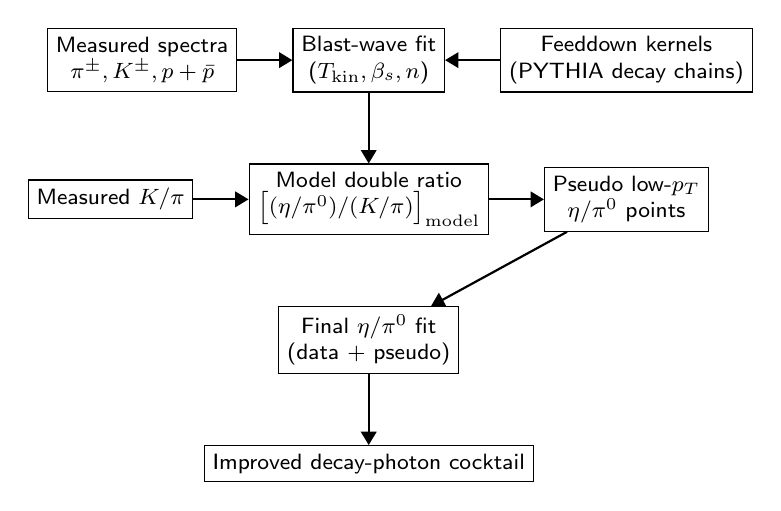
\begin{tikzpicture}[
  node distance=9mm and 7mm,
  box/.style={draw, align=center, inner sep=3pt, font=\sffamily\footnotesize},
  arr/.style={-Triangle, line width=0.8pt}
]
\node[box] (data) {Measured spectra\\$\pi^\pm, K^\pm, p+\bar p$};
\node[box, right=of data] (fit) {Blast-wave fit\\($T_{\mathrm{kin}}, \beta_s, n$)};
\node[box, right=of fit] (kernel) {Feeddown kernels\\(PYTHIA decay chains)};
\node[box, below=of fit] (dr) {Model double ratio\\$\left[(\eta/\pi^0)/(K/\pi)\right]_{\mathrm{model}}$};
\node[box, left=of dr] (kpi) {Measured $K/\pi$};
\node[box, right=of dr] (eta) {Pseudo low-$p_T$\\$\eta/\pi^0$ points};
\node[box, below=of dr] (final) {Final $\eta/\pi^0$ fit\\(data + pseudo)};
\node[box, below=of final] (cocktail) {Improved decay-photon cocktail};

\draw[arr] (data) -- (fit);
\draw[arr] (kernel) -- (fit);
\draw[arr] (fit) -- (dr);
\draw[arr] (kpi) -- (dr);
\draw[arr] (dr) -- (eta);
\draw[arr] (eta) -- (final);
\draw[arr] (final) -- (cocktail);
\end{tikzpicture}
}
\endgroup
\caption{Workflow for constructing a data-constrained low-$p_T$ $\eta/\pi^0$ ratio and propagating it to the decay-photon cocktail in the blast-wave model + feeddown approach.}
\label{fig:workflow}
\end{figure}

\subsection{Flow-Scaling Alternative}
We introduce the flow-scaling method as an alternative cross-check to our core double-ratio method. Using a single effective flow velocity $\beta$, we assume that hadron $p_T$ spectra for species $a$ can be approximated by
\begin{equation}
  \frac{dN_a}{dp_T\,dy} = C_a F(m_T^*)
\end{equation}
where $F$ is a universal scaling function describing the shape and the Lorentz-transformed transverse mass $m_T^*$ is defined as
\begin{equation}
  m_T^* = \gamma (m_T - \beta p_T) \,.
\end{equation}
Based on the measured $\pi$, $K$, $p$ spectra, we determine the optimal flow velocity $\beta$ in the range $0.5 < p_T < 2.5\,\mathrm{GeV}/c$ where spectra are well described by hydrodynamic models.

In the flow-scaling method we can predict the $\eta/K$ ratio as a function of $p_T$ as 
\begin{equation}
  (\eta/K)_\mathrm{flow\text{-}scaling}
  = 
  \frac{F\left(\gamma (\sqrt{m_\eta^2+p_T^2} - \beta p_T)\right)}{F\left(\gamma (\sqrt{m_K^2+p_T^2} - \beta p_T)\right)}, 
\end{equation}
i.e., in this work we assume $C_\eta = C_K$. To compare this result with the $\eta/\pi^0$ ratio as a function of $p_T$ from the double-ratio method, we use the $\pi/\pi^0$ ratio from the double-ratio method according to
\begin{equation}
  \begin{split}
  (\eta/\pi^0)_\mathrm{flow\text{-}scaling}
  &= (\eta/K)_\mathrm{flow\text{-}scaling}\,(\pi/\pi^0)_\text{blast-wave} \\
  &\quad\times \left(K/\pi\right)_{\mathrm{AA,\,meas}} \, .
  \end{split}
  \label{eq:eta_to_pi0_from_eta_to_K}
\end{equation}

% Figure (optional): flow-scaling concept F(x), x = gamma(m_T - beta p_T)

\section{\boldmath Inputs and Model Ingredients (Pb--Pb $\sqrt{s_{NN}}=2.76$ TeV, 0--10\%)}

\subsection{\boldmath Simultaneous Fit to $\pi$, $K$, and $p$ Spectra}
We apply our method to $\pi$, $K$, and $p$ spectra measured by ALICE at $\sqrt{s_{NN}}=2.76$ TeV in the 0--10\% centrality class. The simultaneous blast-wave fit including feeddown is shown in Fig.~\ref{fig:fit_blastwave_2p76_0_10}. The relative normalizations of the $\pi$, $K$, and $p$ spectra are left as free parameters. Even though feeddown is included, the model underestimates the pion spectrum at low $p_T$. This has been observed to be a rather generic feature when describing pion spectra with hydrodynamic models~\cite{Lu:2024shm,Nijs:2020roc}. In the present analysis, however, we are primarily concerned with $p_T \gtrsim 0.5\,\mathrm{GeV}/c$, so this low-$p_T$ mismatch is not a limiting issue for our strategy.
\begin{figure}[t]
\centering
\includegraphics[width=\columnwidth]{./figures/fit_blastwave_combined_2p76TeV_0_10.pdf}
\caption{Simultaneous blast-wave + feeddown fit to the measured $\pi^\pm$, $K^\pm$, and $(p+\bar p)$ spectra in 0--10\% Pb--Pb collisions at $\sqrt{s_{NN}}=2.76$ TeV \cite{ALICE:2014juv}. For visibility, the $K^\pm$ and $(p+\bar p)$ spectra are scaled by factors of 8 and 30, respectively.}
\label{fig:fit_blastwave_2p76_0_10}
\end{figure}

\subsection{Double Ratio from Blast-Wave Model with Feeddown}

The double ratio $(\eta/\pi^0)/(K^+/\pi^+)$ for the blast-wave parameters obtained from the fit to the $\pi$, $K$, and $p$ spectra is shown in Fig.~\ref{fig:model_double_ratio_2p76_0_10}. We also show the $\eta/K^+$ ratio and the $\pi^+/\pi^0$ separately. The larger $\pi^0$ yield at low $p_T$ compared to $\pi^+$ is related to isospin-violating decays of the $\eta$ meson.

Propagating the blast-wave fit covariance yields a double-ratio uncertainty band smaller than the plotted line width and it is therefore not shown in Fig.~\ref{fig:model_double_ratio_2p76_0_10}.

\begin{figure}[t]
\centering
\includegraphics[width=\columnwidth]{./figures/double_ratio_feeddown_2p76TeV_0_10.pdf}
\caption{Feeddown-based blast-wave model double ratio $(\eta/\pi^0)/(K^+/\pi^+)$ for 0--10\% Pb--Pb collisions at $\sqrt{s_{NN}}=2.76$ TeV (solid line). The component ratios $\eta/K^+$ (dashed) and $\pi^+/\pi^0$ (dotted) are shown for reference.}
\label{fig:model_double_ratio_2p76_0_10}
\end{figure}

\section{Cross-Checks and Systematic Uncertainties}
\label{sec:systematics}
To estimate the accuracy of the predicted $(\eta/\pi^0)/(K^+/\pi^+)$ in the blast-wave model with feeddown, we compare our result with a full hydrodynamic simulation with the FluiduM code \cite{Floerchinger:2018pje}, using separate chemical and kinetic freeze-out in the partial chemical equilibrium approach. In FluiduM, the contribution of decays of short-lived hadrons to hadron spectra is obtained with FastReso \cite{Mazeliauskas:2018irt}. The parameters for 0--10\% Pb--Pb collisions at $\sqrt{s_{NN}}=2.76$ TeV ($T_\mathrm{chem} = 141~\mathrm{MeV}$, $T_\mathrm{kin} = 122~\mathrm{MeV}$, $\mathrm{Norm}_{2.76} = 36$, and $\tau_{0,2.76} = 0.76~\mathrm{fm}/c$) are taken from \cite{Vermunt:2023zsk} (solid black line in Fig.~\ref{fig:systematics_summary_2p76_0_10}). $\mathrm{Norm}_{2.76}$ is an overall normalization factor for the initial energy density profile and $\tau_{0,2.76}$ is the initial time for the hydrodynamic evolution.

Moreover, we vary the chemical freeze-out temperature $T_\mathrm{chem}$ in the statistical-model particle densities used for feeddown normalization in the blast-wave model approach from 156~MeV to 136~MeV and 176~MeV. The resulting change of the double ratio is shown as green dashed lines in Fig.~\ref{fig:systematics_summary_2p76_0_10}.

As a further check of the robustness of our method, we perform a blast-wave fit without feeddown (noFD) and construct an $\eta/\pi^0$ prediction by replacing the flow-scaling input for $\eta/K$ in Eq.~\ref{eq:eta_to_pi0_from_eta_to_K} with $(\eta/K)_{\mathrm{blast\text{-}wave,\ noFD}}$. This avoids the known low-$p_T$ bias in $\pi^+/\pi^0$ from a fully no-feeddown approach and provides a fairer comparison of the no-feeddown impact on the $\eta/K$ part of the method. We also compare the blast-wave model prediction for the double ratio with the flow-scaling method as an alternative way to predict hadron spectra in the presence of strong radial flow.

We consider the comparison with FluiduM as the main benchmark for the accuracy of our method. Based on the observed deviations, we assign a relative uncertainty of $\pm 5\%$ to the double ratio from our blast-wave + feeddown approach. This is shown as a gray band in Fig.~\ref{fig:systematics_summary_2p76_0_10} and propagated to the final $\eta/\pi^0$ result as a systematic uncertainty for the low-$p_T$ extrapolation. For other collision systems or centralities, this uncertainty should be re-evaluated using corresponding benchmark studies.

\begin{figure}[t]
\centering
\includegraphics[width=\columnwidth]{./figures/systematics_summary_2p76TeV_0_10.pdf}
\caption{Summary of systematic variations for the double ratio $(\eta/\pi^0)/(K^+/\pi^+)$ in 0--10\% Pb--Pb collisions at $\sqrt{s_{NN}}=2.76$ TeV. The baseline blast-wave result with feeddown is compared with a no-feeddown hybrid comparator, the flow-scaling alternative, and variations of $T_{\mathrm{chem}}$. The gray band indicates the fixed uncertainty envelope used in the summary scan.}
\label{fig:systematics_summary_2p76_0_10}
\end{figure}

\section{\boldmath Results: $\eta/\pi^{0}(p_T)$ in 0--10\% Pb--Pb at 2.76 TeV}

We can now predict the $\eta/\pi^0$ ratio for $p_T \lesssim 3~\mathrm{GeV}/c$ by multiplying the blast-wave double ratio with the measured charged $K/\pi$ ratio. The resulting pseudo-data points are then fitted together with the measured $\eta/\pi^0$ data to obtain a parameterization over the full $p_T$ range. The resulting curve and the associated systematic uncertainty band for the low-$p_T$ extrapolation are shown in Fig.~\ref{fig:eta_to_pi0_2p76_0_10}. We compare our result to the Ren--Drees method and find that both approaches give very similar predictions for the low-$p_T$ $\eta/\pi^0$ ratio. In Sec.~\ref{sec:feeddown_structure}, we show that the feeddown contribution to both the $\eta$ spectrum (Fig.~\ref{fig:feeddown_fractions_eta}) and the $K$ spectrum (Fig.~\ref{fig:feeddown_fractions_k_plus}) is significant. The overall feeddown contribution to the $\eta$ spectrum is about 40\% for $p_T < 3~\mathrm{GeV}/c$, and for the $K$ spectrum it is slightly larger. The similar size of the feeddown contribution for $K$ and $\eta$ may help explain why the Ren--Drees method, which does not explicitly include feeddown, gives a prediction for the low-$p_T$ $\eta/\pi^0$ ratio similar to that of our blast-wave fit with feeddown.

The uncertainty band around the fitted $\eta/\pi^0$ parameterization is constructed as follows. For $p_T \lesssim 2.5~\mathrm{GeV}/c$, we use the assigned relative uncertainty of $\pm 5\%$ for the double-ratio method discussed in Sec.~\ref{sec:systematics}. In the intermediate region $2.5 < p_T < 4.0~\mathrm{GeV}/c$, where no pseudo-data points are imposed, the relative uncertainty is interpolated smoothly to the average relative experimental uncertainty of the measured $\eta/\pi^0$ data in the range $3 < p_T < 4~\mathrm{GeV}/c$. For $4 < p_T < 5~\mathrm{GeV}/c$, the band is interpolated linearly to a constant asymptotic uncertainty of 5\%, which is then used for $p_T > 5~\mathrm{GeV}/c$. This construction is intended as a pragmatic uncertainty model that connects the low-$p_T$ model-constrained region smoothly to the experimentally constrained and high-$p_T$ regions.

Figure~\ref{fig:eta_to_pi0_2p76_0_10} also shows a parameterization of the $\eta/\pi^0$ ratio in pp collisions using the parameterization of Eq.~\ref{eq:eta_to_pi0_parameterization}. The parameters used here were obtained from a fit to pp data at different energies while keeping the high-$p_T$ ratio $r = 0.487 \pm 0.024$ \cite{Ren:2021pzi} and the radial flow velocity $\beta = 0$ fixed (see Fig.~\ref{fig:eta_to_pi0_pp_pA_fit}). The difference between the pp parameterization and the Pb--Pb result at low $p_T$ illustrates the significant effect of radial flow on the $\eta/\pi^0$ ratio in heavy-ion collisions.  

\begin{figure}[t]
\centering
\includegraphics[width=\columnwidth]{./figures/eta_to_pi0_data_2p76TeV_0_10.pdf}
\caption{$\eta/\pi^0$ in 0--10\% Pb--Pb collisions at $\sqrt{s_{NN}}=2.76$ TeV \cite{ALICE:2018mdl}. Measured points are combined with pseudo-data constraints from the double-ratio method and fitted with the flow-inspired parameterization of Eq.~\ref{eq:eta_to_pi0_parameterization}. The shaded band indicates the systematic uncertainty model used for the low-$p_T$ extrapolation. We also show a fit of only the measured $\eta/\pi^0$ points without the low-$p_T$ pseudo-data constraints (dark gray dashed line). The parameterization of the $\eta/\pi^0$ ratio in pp collisions is shown for reference (light gray dashed line) and illustrates the significant effect of radial flow on the $\eta/\pi^0$ ratio in heavy-ion collisions. The blast-wave + feeddown prediction shows good agreement with the Ren--Drees prediction (gray points).}
\label{fig:eta_to_pi0_2p76_0_10}
\end{figure}

\section{Implications for the Decay-Photon Cocktail}

A reduction and improved control of the $\eta/\pi^0$ uncertainty, aimed at enabling more precise direct-photon measurements at low $p_T$, constitutes the primary motivation of this study. The impact of the $\eta/\pi^0$ uncertainty on the direct-photon measurement is illustrated in Figure~\ref{fig:decay_photon_cocktail_fractions_2p76_0_10}. The dominant contributions to the decay-photon background arise from $\pi^0$, $\eta$, and $\omega$ meson decays.

Analogous to the feeddown treatment in the blast-wave + feeddown model, we construct the decay-photon cocktail using precomputed decay-photon kernels. For each hadron with a direct-photon decay branch, the corresponding kernel is generated with PYTHIA~8. The total decay-photon $p_T$ spectrum is then obtained by folding these two-dimensional kernels with the parent-hadron $p_T$ spectra. In this framework, we include contributions from $\pi^0$, $\eta$, $\omega$, $\eta'$, $\rho^0$, $\Sigma^0$, and $\bar{\Sigma}^0$. The $\pi^0$ parameterization is taken from \cite{ALICE:2018mdl}. For hadrons other than $\pi^0$ and $\eta$, we use flow-scaling parameterizations.

Although this method does not represent a substantial conceptual improvement over a standard full Monte Carlo decay simulation, it offers significant practical advantages. In particular, it enables a rapid and flexible evaluation of how variations in the parameterizations of the hadron $p_T$ spectra propagate to the decay-photon cocktail and, consequently, to the extracted direct-photon signal.

The upper panel of Fig.~\ref{fig:decay_photon_cocktail_fractions_2p76_0_10} shows the fractional contributions of selected parent particles to the decay-photon cocktail in 0--10\% Pb--Pb collisions at $\sqrt{s_{NN}}=2.76$ TeV. Clearly, the $\pi^0$ and $\eta$ decay contributions dominate the cocktail across the entire $p_T$ range. On a linear scale, one can see the small contribution of the $\omega$ meson, while all other contributions are negligible. The lower panel illustrates the impact of the $\eta$-related uncertainty on the direct-photon signal, compared with the direct-photon excess predicted by the model calculation of Ref.~\cite{Gale:2021emg}. The total predicted direct-photon signal, comprising prompt, pre-equilibrium, and thermal photons, is shown, along with the thermal-photon contribution separately, for the scenario without suppression from quarks initially being out of chemical equilibrium. Quantitatively, at $p_T \approx 1~\mathrm{GeV}/c$, the $\eta$-related uncertainty corresponds to about 10\% of the expected direct-photon signal. This comparison underscores the importance of constraining the $\eta/\pi^0$ ratio for improving the precision of direct-photon measurements in heavy-ion collisions.

\begin{figure}[t]
\centering
\includegraphics[width=\columnwidth]{./figures/decay_photon_cocktail_fractions_2p76TeV_0_10.pdf}
\caption{Decay-photon cocktail fractions for 0--10\% Pb--Pb collisions at $\sqrt{s_{NN}}=2.76$ TeV. Upper panel: fractional decay-photon contributions from $\pi^0$, $\eta$, and $\omega$. The uncertainty of the $\eta$ contribution is shown as a shaded band. Lower panel: $\eta$-related uncertainty of the decay-photon background compared with the direct-photon signal predicted in Ref.~\cite{Gale:2021emg}.}
\label{fig:decay_photon_cocktail_fractions_2p76_0_10}
\end{figure}

\section{Conclusions}

We have presented a practical, data-driven approach to predict the $\eta/\pi^0$ ratio at low $p_T$ ($p_T \lesssim 3~\mathrm{GeV}/c$), based on the measured charged $K/\pi$ ratio and model input from a blast-wave framework with feeddown contributions. After determining the model parameters from fits to the measured $\pi$, $K$, and $p$ spectra, we construct the $(\eta/\pi^0)/(K^+/\pi^+)$ double ratio and use it to obtain pseudo-data constraints for $\eta/\pi^0$. This method is expected to be useful for future direct-photon and dilepton analyses in heavy-ion collisions, where precise hadron background estimates are essential. We have illustrated this impact for direct photons in Pb--Pb collisions at $\sqrt{s_{NN}}=2.76$~TeV.

The double-ratio method yields predictions that are numerically close to the Ren--Drees approach. This agreement is non-trivial and supports the practical validity of the Ren--Drees method in the studied kinematic range. At the same time, by explicitly modeling the feeddown contributions to the $\eta$ and $K$ spectra and accounting for the particle-mass dependence of radial flow, the present framework makes the underlying ingredients explicit. The flow-scaling cross-check can be viewed as a practical extension of traditional $m_T$ scaling in the presence of strong radial flow and can serve as a more physically motivated baseline for modeling $p_T$ spectra of heavier hadrons in decay-cocktail calculations. In summary, our approach allows for a controlled extrapolation of the $\eta$ meson spectrum toward low $p_T$, addressing a typical bottleneck in direct-photon and dielectron analyses. 

\section*{Code Availability}
The analysis code used to generate the results and figures presented in this work is publicly available at \url{https://github.com/reygers/eta-pi0-blastwave-feeddown} \cite{reygers_eta_pi0_blastwave_feeddown_2026}. Setup instructions and the public analysis workflow are documented in the repository README.

\appendix

\section{\boldmath $\eta/\pi^0$ parameterization in pp collisions}
Fig.~\ref{fig:eta_to_pi0_pp_pA_fit} shows how the $\eta/\pi^0$ parameterization for pp collisions used in this paper is obtained from a fit to pp data at $\sqrt{s}=7~\mathrm{TeV}$ \cite{ALICE:2012wos}, $\sqrt{s}=8~\mathrm{TeV}$ \cite{ALICE:2017ryd}, and $\sqrt{s}=13~\mathrm{TeV}$ \cite{ALICE:2024vgi}, as well as fixed-target p--Be data at a beam momentum of 450~GeV/$c$. The $\eta/\pi^0$ ratio as a function of $p_T$ is found to be approximately independent of the center-of-mass energy \cite{Ren:2021pzi}. The data are fitted using Eq.~\ref{eq:eta_to_pi0_parameterization}. The high-$p_T$ $\eta/\pi^0$ value is fixed to $r=0.487$ reported in \cite{Ren:2021pzi}, and the radial-flow velocity is set to $\beta = 0$.

\begin{figure}[t]
\centering
\includegraphics[width=\columnwidth]{./figures/eta_to_pi0_pp_pA_fit.pdf}
\caption{Fit of the $\eta/\pi^0$ parameterization to pp and p--A reference data (pp at 7, 8, and 13 TeV, and p--Be at 450 GeV/$c$). The fit uses the same flow-inspired functional form employed in this work for the $\eta/\pi^0$ description. The high-$p_T$ value is fixed to $r=0.487$ and the radial-flow parameter is set to $\beta=0$.}
\label{fig:eta_to_pi0_pp_pA_fit}
\end{figure}

\section{\boldmath $\eta/\pi^0$ from $m_T$ scaling}
As an additional baseline, we compare our data-driven $\eta/\pi^0$ result with the traditional $m_T$-scaling approach. In this approach, invariant yields of different hadron species are assumed to have the same functional dependence on transverse mass, up to a constant normalization factor. Using a parameterization $h_{\pi^0}(p_T)$ of the invariant neutral pion $p_T$ spectrum, this corresponds to
\begin{equation}
\left(\frac{\eta}{\pi^0}\right)_{m_T}(p_T)
=
C_{\eta/\pi^0}\,
\frac{h_{\pi^0}\!\left(\sqrt{p_T^2+m_\eta^2-m_{\pi^0}^2}\right)}
     {h_{\pi^0}(p_T)} \, .
\end{equation}
In this work, we fix the normalization to the high-$p_T$ value $C_{\eta/\pi^0}=0.487$.

Figure~\ref{fig:eta_pi0_mt_vs_flow_2p76_0_10} compares, for 0--10\% Pb--Pb collisions at $\sqrt{s_{NN}}=2.76$~TeV, the $m_T$-scaling prediction with the measured $\eta/\pi^0$ data and with our fit based on measured plus pseudo-data constraints. The $m_T$-scaling curve is constructed using the $\pi^0$ parameterization from \cite{ALICE:2018mdl}. While $m_T$ scaling provides a useful reference, it does not reproduce the full low-$p_T$ behavior expected in the presence of strong radial flow.


\begin{figure}[t]
\centering
\includegraphics[width=\columnwidth]{./figures/eta_pi0_mt_vs_flow_2p76TeV_0_10.pdf}
\caption{Comparison of the $m_T$-scaling prediction (green) and the fitted $\eta/\pi^0$ parameterization based on measured plus pseudo-data constraints (orange) for 0--10\% Pb--Pb collisions at $\sqrt{s_{NN}}=2.76$~TeV. Measured $\eta/\pi^0$ points are shown in black; the gray dashed line indicates the pp reference parameterization.}
\label{fig:eta_pi0_mt_vs_flow_2p76_0_10}
\end{figure}

\section{Flow scaling function}

For 0--10\% central Pb--Pb collisions at $\sqrt{s_{NN}}=2.76$~TeV, the flow-scaling construction gives the best collapse of the measured $\pi$, $K$, and $p$ spectra for an effective radial-flow velocity of $\beta = 0.6972$. The value of $\beta$ is obtained from a scan that minimizes the spread of the scaled hadron spectra in the fit interval $0.5 < p_T < 2.5~\mathrm{GeV}/c$. The corresponding scaling function $F(m_T^*)$ is shown in Fig.~\ref{fig:flow_scaling_collapse_2p76_0_10}, where
\begin{equation}
  m_T^*=\gamma(m_T-\beta p_T)
\end{equation}
denotes the transverse mass in the source rest system. The collapsed yields are parameterized with the Tsallis-like form
\begin{equation}
F(m_T^*) \propto \left(1 + \frac{m_T^*}{n T}\right)^{-n} \,.
\end{equation}
In Fig.~\ref{fig:flow_scaling_collapse_2p76_0_10} we show the range $0.2 \le m_T^* \le 1.4$, which covers the kinematic region relevant for the low-$p_T$ $\eta/\pi^0$ extrapolation. This smooth $F(m_T^*)$ parameterization is used only as a cross-check input in the systematic study; its deviation from the core blast-wave + feeddown result contributes to the assigned method uncertainty shown in Fig.~\ref{fig:systematics_summary_2p76_0_10}.

\begin{figure}[t]
\centering
\includegraphics[width=\columnwidth]{./figures/flow_scaling_collapse_2p76TeV_0_10.pdf}
\caption{Flow-scaling collapse plot for 0--10\% Pb--Pb collisions at $\sqrt{s_{NN}}=2.76$ TeV. The scaled $\pi$, $K$, and $p$ data are shown as a function of $m_T^* = \gamma(m_T-\beta p_T)$, i.e.\ the transverse mass in the source rest system, together with the smooth fit used in the flow-scaling cross-check.}
\label{fig:flow_scaling_collapse_2p76_0_10}
\end{figure}

\section{\boldmath Feeddown Structure for $\eta$ and $K^+$}
\label{sec:feeddown_structure}

The feeddown compositions are shown in Fig.~\ref{fig:feeddown_fractions_eta} for the $\eta$ meson and in Fig.~\ref{fig:feeddown_fractions_k_plus} for the $K^+$ meson. The feeddown is obtained from the PYTHIA 8 particle list for particles up to a mass of $m=2~\mathrm{GeV}/c^2$ and with proper decay length $c\tau < 1~\mathrm{mm}$. The primary-particle spectra are modeled in the blast-wave + feeddown approach with parameters obtained from fits to the $\pi$, $K$, and $p$ spectra in 0--10\% Pb--Pb collisions at $\sqrt{s_{NN}}=2.76$~TeV.

\begin{figure}[t]
\centering
\includegraphics[width=\columnwidth]{./figures/feeddown_fractions_eta.pdf}
\caption{Primary and feeddown fractions for $\eta$ as a function of $p_T$ in the blast-wave + feeddown setup used in this work. The ten most dominant parent contributions are shown together with the primary component.}
\label{fig:feeddown_fractions_eta}
\end{figure}

\begin{figure}[t]
\centering
\includegraphics[width=\columnwidth]{./figures/feeddown_fractions_k_plus.pdf}
\caption{Primary and feeddown fractions for $K^+$ as a function of $p_T$ in the blast-wave + feeddown setup used in this work. The ten most dominant parent contributions are shown together with the primary component.}
\label{fig:feeddown_fractions_k_plus}
\end{figure}

\clearpage

\begin{acknowledgments}
This work has been supported by the DFG (German Research Foundation) --- Project No.\ 273811115 --- SFB 1225 ISOQUANT.
AM is supported by the DFG through the Emmy Noether Programme (Project No.\ 496831614).
AK is supported by the U.S. Department of Energy, Office of Science, Office of Nuclear Physics, grant No. DE-FG02-05ER41367.
We wish to acknowledge helpful discussions with Ana Marin, Ilya Fokin, and Johanna Stachel. We used OpenAI Codex to assist with code generation based on human-written prompts. All scientific results, validations, and interpretations were performed by the authors.

\end{acknowledgments}

\bibliography{master}% Produces the bibliography via BibTeX.

\end{document}


%
% ****** End of file apssamp.tex ******
